% !TEX root = ../thesis-main.tex
\section{Реализация инструмента генерации программ}

\subsection{Используемые технологии}

Для разработки инструмента был выбран язык программирования Kotlin \cite{kotlin}. Это язык
программирования, разработанный компанией JetBrains в 2010 году. Основными
преимуществами этого языка программирования являются:
\begin{itemize}
    \item Кроссплатформенность
    \item Возможность интеграции с различными популярными системами сборки
          (Maven, Gradle, etc.)
    \item Возможность интеграции с java без переписывания имеющегося кода
    \item Возможность создания DSL.
\end{itemize}

Для автоматизации развертывания системы генерации, поддерживания окружения для хранилища и
системы проверки используются технологии Docker \cite{docker} и docker-compose \cite{docker-compose}.
Благодаря Docker можно создать изолированное окружение (контейнер) для компонента, а docker-compose
позволяет объединять контейнеры в единую локальную сеть. В данном проекте созданы отдельные
контейнеры для базы данных и веб-сервера.


\subsubsection{Менеджер шаблонов}
Для хранения и пересылки шаблонов была добавлена поддержка конвертации шаблона в формат JSON~---
один из самых распространенных форматов обмена данных, который также может использоваться и для
хранения информации (см \ref{db}). Из-за сложной структуры классов,
в виде экземпляров которых представляется шаблон (\ref{template-classes}), для сериализации шаблонов в
JSON была выбрана библиотека \texttt{Kotlinx.serialization} \cite{kotlinx-serialization},
которая поддерживает сериализацию объектов языка программирования Kotlin и умеет работать
с наследованием и полиморфизмом.

Для отправки запросов на создание и удаление через Интернет был использован
Http~-клиент фреймворка Ktor \cite{ktor}, так как данный клинт поддерживает
сериализацию тела запроса (и ответа) с помощью \texttt{Kotlinx.serialization}.

\subsubsection{Веб-сервер}
Для реализации веб-сервера в связи с использованием для сериализации \texttt{Kotlinx.serialization}
было принято решение использовать Http~-сервер фреймворка Ktor \cite{ktor}, который поддерживает
данный способ сериализации запросов, а также имеет простой и элегантный API и возможность расширения
с помощью плагинов.

\subsubsection{База данных}
\label{db}
Так как шаблоны программ конвертируются и передаются в формате JSON, то было принято решение
переиспользовать имеющуюся логику и хранить их также в этом формате. В данном проекте используется
\texttt{MongoDB}~\cite{mongodb}~--- база данных, которая работает именно с форматом JSON.

Для работы с \texttt{MongoDB} из серверного кода была выбрана библиотека \texttt{kmongo}. Данная
библиотека является самой популярной библиотекой для работы с \texttt{MongoDB} из языка
\texttt{Kotlin}, также она поддерживает конвертацию в JSON и обратно с помощью
\texttt{Kotlinx.serialization}, что также упрощает работу с шаблонами.

Поля, которые хранятся в соответствующих коллекциях, описаны в \ref{db-model}. Однако в
данной библиотеке отсутствует поддержка хранение сырых байтов в базе данных, поэтому для
хранения изображения кода в базе байты изображения, с помощью алгоритма Base64\cite{rfc4648},
преобразуются в строку и в таком виде сохраняются в базу.

\subsubsection{Исполнитель программ}
Для компиляции (при необходимости), выполнения, форматирования кода и генерации изображений используются
отдельные программы, запускающиеся во внешнем окружении. По соображениям безопасности и для
ограничения нагрузки на инфраструктуру, на которой работает сервер, одновременно может работать
только один исполнитель, для этого в веб-сервере код, выполняющий программы во внешнем окружении,
запускается под блокировкой мьютекса. Для файлов, создаваемых во время выполнения, выделен
отдельный каталог.

Для генерации изображений по коду используется библиотека\\
\texttt{python-pygments}\cite{pygments} и поставляемая
с ней программа \texttt{pygmentize}. Данная библиотека написана на языке программирования
Python\cite{python} и поддерживает большинство популярных языков
программирования\cite{pygments-languages}. Изображения генерируются в формате png.

Для остальных задач из списка используются утилиты, специфичные для конкретного языка программирования.
Пример таких утилит для языка программирования Python\cite{python}:

\begin{itemize}
    \item Утилита для форматирования: \texttt{autopep8}\cite{autopep8}
    \item Компилятор: компиляция не требуется
    \item Утилита для выполнения кода: стандартный интерпретатор \texttt{python} версии 3.10
\end{itemize}

Для форматирования, генерации изображения и компиляции установлено ограничение по времени в 10 секунд,
для выполнения кода~--- 30 секунд.

\subsection{Шаблоны программ}
\subsubsection{Внутреннее представление шаблона} \label{template-classes}
Объект шаблона представляет собой экземпляр класса \texttt{ProgramTemplate},
параметризованного тэгом, соответствующим языку или группе языков программирования с
общими свойствами. Все упомянутые далее классы также параметризованы тэгом.

Сам тэг предоставляет собой сущность \texttt{object} (представляющую собой
singleton \cite{singleton}) языка программирования Kotlin,
наследованный от класса \texttt{ProgramLanguageTag} и набора интерфейсов, соответствующих
особенностям языка. Примером такого интерфейса является \texttt{DynamicTyping},
обозначающий, что данный язык программирования имеет динамическую типизацию
\cite{dynamic-typing}. С точки зрения синтаксиса это, к примеру, означает, что не
обязательно указывать типы аргументов при объявлении функции.

Внутри данного объекта содержится объект класса\\ \texttt{ProgramGlobalTemplate}.
Этот и парный к нему класс \texttt{ProgramLocalTemplate} сопоставляются
глобальной и локальной области видимости. Внутри объектов данных классов
содержится список элементов программы, находящихся в соответствующей области
видимости.

Примеры элементов программы:
\begin{itemize}
    \item \texttt{VariableTemplate} --- ссылка на переменную.
    \item \texttt{AssigmentTeamplate}, \texttt{VariableDefinitionTemplate} ---
          присвоение значения в переменную и объявление переменной.
    \item \texttt{FunctionDefinitionTemplate}, \texttt{FunctionCallTemplate} ---
          объявление и вызов функции.
    \item \texttt{IfElseInstuctionTemplate}, \texttt{WhileTemplate} --- условные
          ветвления и циклы.
    \item \texttt{ProgramConstantTemplate} --- общий класс для разных типов констант. Примеры наследников
          данного класса:
          \begin{itemize}
              \item \texttt{NumConstantTemplate}, \texttt{StringConstantTemplate} ---
                    обычные числовые и строковые константы.
              \item \texttt{RandomNumConstantTemplate}, \texttt{RandomStringConstantTemplate},\\
                    \texttt{RandomChoiceConstant}, \texttt{RandomChoiceStringConstant}
                    --- случайные числовые и строковые значения, которые генерируются и транслируются
                    в обычные константы во время преобразования шаблона в промежуточное предоставление.
                    Первые два класса генерируют значения согласно переданным параметрам, последние два ---
                    выбирая из фиксированного списка значений.
              \item \texttt{NumAttributeRef}, \texttt{StringAttributeRef} --- значения атрибутов,
                    передаваемых при конвертации в промежуточное представление.
          \end{itemize}
    \item \texttt{ProgramConstantListTemplate} --- общий класс для списка констант, аналогично
          \texttt{ProgramConstantTemplate}.
    \item \texttt{ProgramExpressionTemplate} --- общий класс для выражений. Является,
          в частности, предком классов \texttt{ProgramConstantTemplate},\\ \texttt{ProgramConstantListTemplate}
          и \texttt{VariableTemplate}. Также его наследником является
          \texttt{BinOpExpressionTemplate} --- класс, соответствующий бинарным операциям.
    \item \texttt{RepeatLocalScopeTemplate}, \texttt{RepeatGlobalScopeTemplate} ---
          служебные классы, которые при генерации промежуточного представления повторяют
          переданный \texttt{scope} заданное число раз. При генерации внутреннего
          \texttt{scope} также можно получить доступ к номеру текущей итерации.
          Также есть классы \texttt{ForeachRepeatLocalScopeTemplate} и \\
          \texttt{ForeachRepeatGlobalScopeTemplate}, которые перебирают и передают в
          функцию-построитель элементы списка. Подробнее об этом в \ref{template-constuct}.
\end{itemize}

\subsubsection{Конструирование шаблонов} \label{template-constuct}

Для создания шаблонов программ в дипломном проекте используется язык программирования Kotlin \cite{kotlin}.
Шаблон представляет собой объект языка программирования Kotlin, созданный с помощью
специальных функций-построителей. Каждая такая функция соответствует классу из
\ref{template-classes} либо строит его часть.

Функции, соответствующие инструкциям,
добавляют созданный объект в \texttt{scope}, а соответствующие выражениям --- возвращают
сгенерированный объект. Данная особенность хорошо видна на примере функций
\texttt{funcCall} и \texttt{addFuncCall}. Так как вызов функции может быть как и
самостоятельной инструкцией, так и частью выражения, то первая функция возвращает объект
и предназначена для использования в выражениях, а вторая --- добавляет вызов в список
элементов \texttt{scope}.

Пример кода, конструирующего шаблон:
\begin{minted}[]{kotlin}
    val task = ProgramTemplate<PythonTag> {
        val xVar = variable("x")
        val stringLen = randomNumConstant(10, 20)
        val randomString = randomStringConstant(stringLen)
        xVar setTo randomString
        `if`(funcCall("len", xVar) lt constant(15)) {
            addFuncCall("print", constant("small"))
        }.`else` {
            addFuncCall("print", constant("long"))
        }
    }
\end{minted}

% \clearpage
Внутреннее представление результата конструирования:
\begin{figure}[ht]
    \begin{center}
        \scalebox{0.55}{
            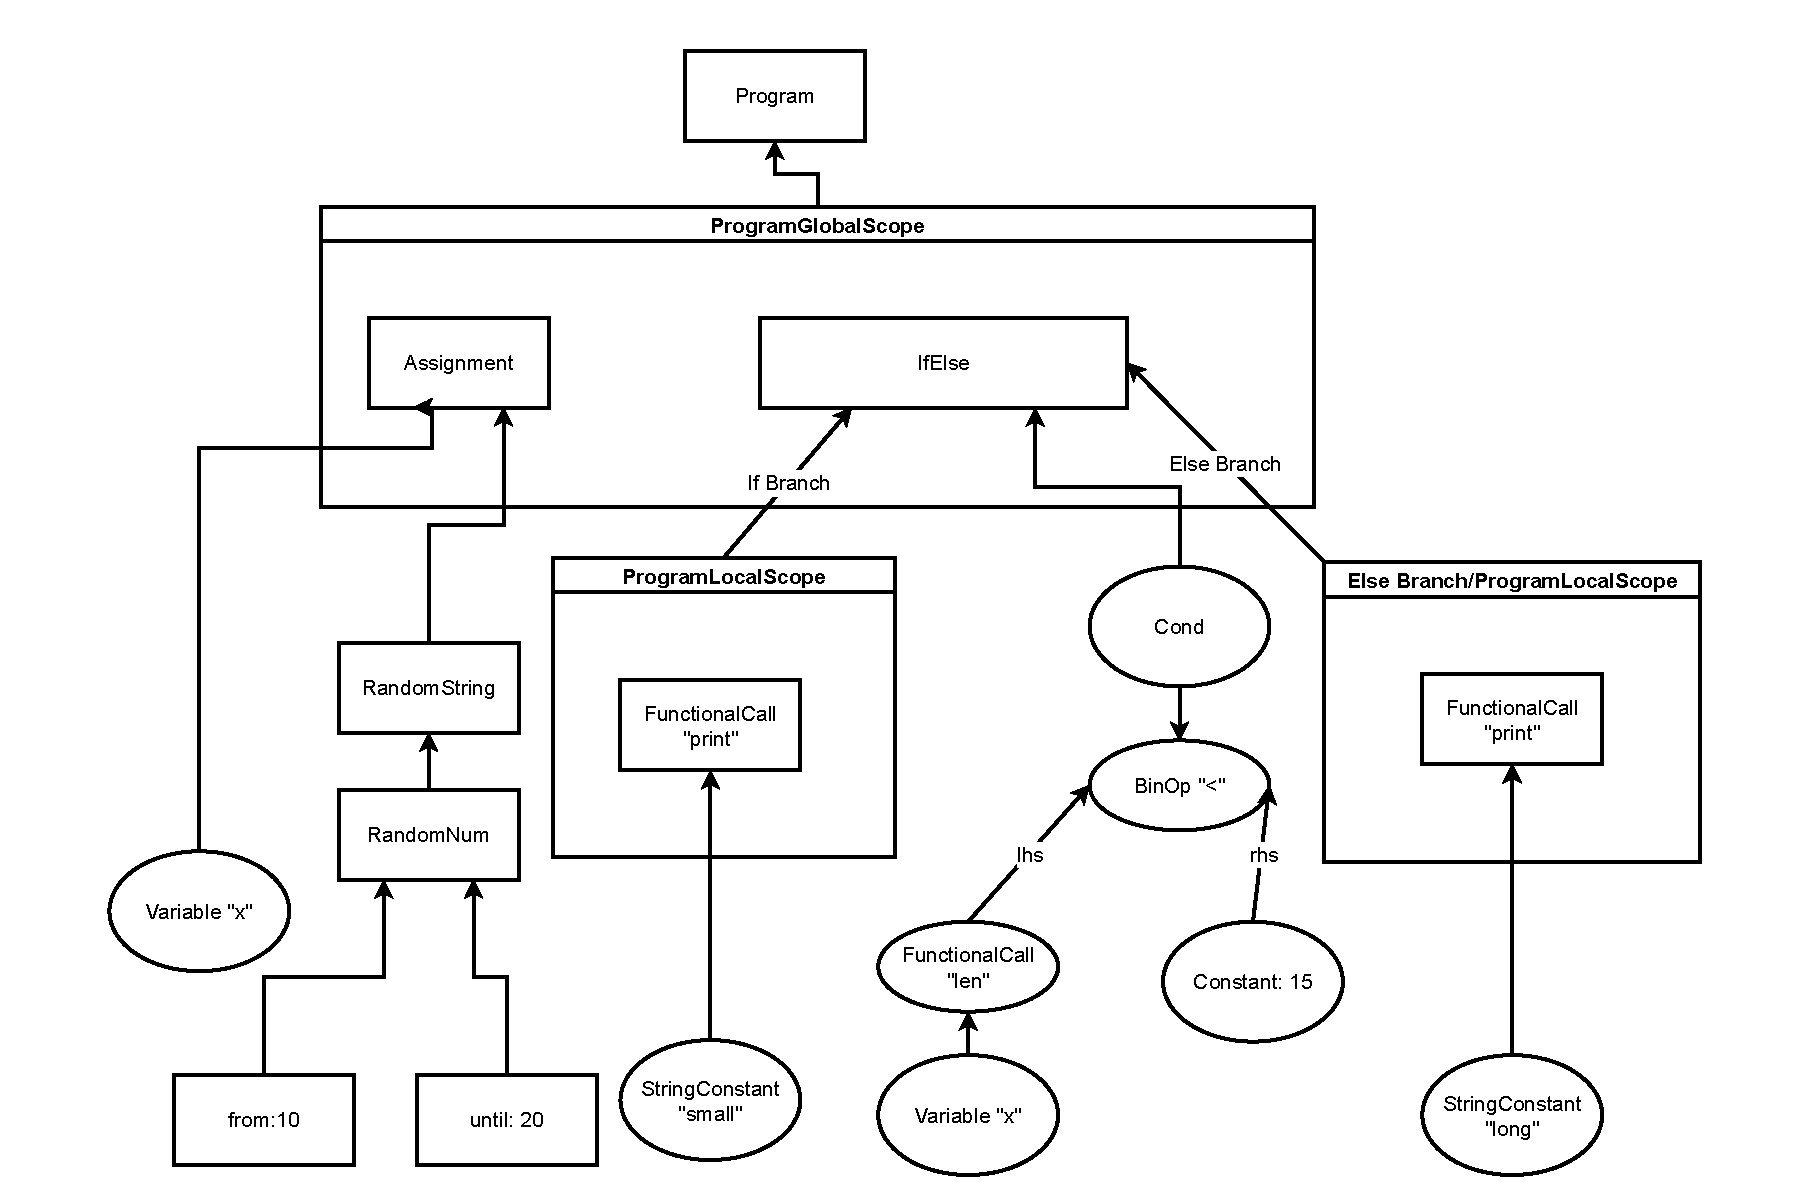
\includegraphics{images/class_tree.pdf}
            % \includesvg[inkscapelatex=false]{images/architecture.drawio.svg}
        }
        \caption{\label{class_tree} Внутреннее представление шаблона}
    \end{center}
\end{figure}
% \clearpage

Благодаря возможностям языка Kotlin \cite{kotlin-dsl}, можно воспроизводить в шаблоне древовидную структуру, где параметры
функции --- это параметры в вершине AST, а последний аргумент (ламбда-функция, переданная за пределами скобок)
описывает поддерево. Это используется в функциях, которые создают новый \texttt{scope}, к примеру
функции \texttt{`if`}, \texttt{`elif`}, \texttt{`else`}, \texttt{`while`},
\texttt{addFunctionalDef}. Также это используется в функциях, которые конструируют
служебные классы.
Примером такого класса и соответствующей ему функции может являться \texttt{RepeatLocalScopeTemplate} и
соответствующая ему функция \texttt{repeat}, которая позволяет повторить несколько раз генерацию
некоторого куска шаблона. К примеру шаблон
\begin{minted}[]{kotlin}
    repeat(2) { i ->
        addFuncCall("print", i)
    }
\end{minted}

сгенерирует следующий код (для языка Python):

\begin{minted}[]{python}
    print(0)
    print(1)    
\end{minted}

Также в построении используется такая особенность языка Kotlin, как инфиксная
нотация \cite{kotlin-infix}, позволяющая вызывать функции с двумя аргументами как
бинарные операторы, то есть размещать имя функции между аргументами. С помощью
этого можно конструировать присваивания и инициализацию переменной (функция
\texttt{setTo} в примере выше) и бинарные операторы в арифметических выражениях
(\texttt{lt} в примере выше).
% \subsection{Примеры задач}
% \textit{(TODO: добавить примеры задач)}
\subsection{Промежуточное представление (AST)}
Внутреннее предоставление AST практически не отличается от предоставления шаблона,
за исключением того, что в AST отсутствуют служебные вершины, отвечающие за
генерацию случайных данных и обращение к атрибутам.

\subsection{Генерация текста программы}
Для генерации кода на конкретном языке программирования необходимо реализовать
интерфейс \texttt{CodeMapper}, который выглядит следующим образом:
\begin{minted}[fontsize=\small]{kotlin}
    interface CodeMapper<LanguageTag : ProgramLanguageTag> {
        fun generateCode(program: Program<in LanguageTag>): String
    }
\end{minted}
По данному интерфейсу видно, что тип \texttt{Program} (а, соответственно, и
все классы в промежуточном предоставлении) является \textit{контравариантным}
\cite{kotlin-variance}, то есть в данный \texttt{CodeMapper} можно передать как
представление программы на языке Python, так и более общие программы,
предназначенные для трансляции в несколько языков.

\subsection{API}
Для взаимодействия с сервером используется Web API.

Для генерации и получения изображений и текстов программ доступны следующие методы API:

\begin{itemize}
    \item \texttt{/get\_source}~--- получить отформатированный текст программы.
          Возвращает текст программы при наличии задачи (см. передаваемые параметры).
    \item \texttt{/get\_image}~--- получить изображение программы. Возвращает \texttt{html} с изображением.
    \item \texttt{/get\_image\_bytes\_png}~--- получить сырые байты изображения. Используется в ссылке
          в \texttt{html} с изображением.
\end{itemize}

Вышеописанные методы принимают следующие параметры в строке URL:
\begin{itemize}
    \item \texttt{task}~--- имя задачи (шаблона), из которого будет сгенерирована программа.
    \item \texttt{seed}~--- значение, используемое как зерно рандомизации при генерации программы.
    \item Прочие параметры передаются как атрибуты генерации программы из шаблона.
\end{itemize}

Для проверки ответа студента используется метод \texttt{/check\_answer}, принимающий
те же параметры, что и методы генерации кода, а также параметр \texttt{answer},
соответствующий ответу студента. Подробнее о проверке ответов в \ref{check-answer}.

Для управления (добавления и удаления) шаблонами программ доступны следующие методы:
\begin{itemize}
    \item \texttt{/add\_task}~--- добавить задачу. Принимает в теле запроса параметры, описанные в
          \ref{template-db}: имя задачи, тэг и шаблон в формате JSON. Данный метод просто сохраняет
          переданные данные в базу
    \item \texttt{/delete\_task}~--- удалить задачу. Принимает в теле запроса структуру, содержащую
          имя удаляемой задачи, в формате JSON. Данный метод удаляет задачу (шаблон) из базы.

\end{itemize}
% (\textit{TODO: примеры кода})

\subsection{Проверка ответов} \label{check-answer}

Для улучшения интеграции с образовательными платформами в инструмент была добавлена
поддержка проверки ответов студентов. Ответом студента для описываемых задач
является вывод программы при ее выполнении. Для проверки ответа студента
генерируется (или запрашивается из базы данных) реальный вывод программы
(см \ref{executor}). Далее реальный вывод построчно сравнивается с ответом студента,
в качестве результата проверки возвращается процент совпавших строк.